\documentclass[11pt,a4paper]{article}

\usepackage[utf8]{inputenc}
\usepackage[T1]{fontenc}
\usepackage[czech]{babel}
\usepackage{lmodern}
\usepackage[a4paper,margin=2.5cm]{geometry}
\usepackage{amsmath}
\usepackage{booktabs}
\usepackage{tabularx}
\usepackage{enumitem}
\usepackage{xcolor}
\usepackage{graphicx}
\usepackage{tikz}
\usetikzlibrary{arrows.meta,positioning}
\usepackage[hidelinks]{hyperref}

% Části, které je nutné doplnit nebo ověřit ručně (v PDF červeně).
\newcommand{\doplnit}[1]{\textcolor{red}{\textbf{[DOPLNIT: #1]}}}

\setlist{itemsep=2pt,topsep=4pt}
\setlength{\emergencystretch}{3em}

\begin{document}

% ---------------------------------------------------------------- titulní strana
\begin{titlepage}
  \centering
  \vspace*{3cm}
  {\large\bfseries České vysoké učení technické v Praze\par}
  Fakulta elektrotechnická\par
  \vspace{2.5cm}
  {\LARGE\bfseries Bludiště na rotačním stolku\par}
  \vspace{1cm}
  {\large Technická zpráva\par}
  \vspace{2.5cm}
  \raggedright
  \textbf{Autoři:} \doplnit{jména všech tří členů týmu}\\
  \textbf{Předmět:} \doplnit{kód a název předmětu}\\
  \textbf{Zvolená varianta:} C -- trajektorie vyžadující pohyb mimo rovinu, bonus za oba směry otáčení\\
  \textbf{Pracoviště:} Bosch SR450 (4-DoF SCARA), kamera Basler, rotační stolek\\
  \textbf{Datum:} \today
\end{titlepage}

% ---------------------------------------------------------------- abstrakt
\begin{abstract}
Zpráva popisuje řešení, ve kterém průmyslový robot Bosch SR450 provlékne obruč bludištěm
umístěným na otáčejícím se stolku. Poloha a otáčení desky s bludištěm se určí z kamery pomocí
dvou ArUco značek. Robot pak předem spočítá časový plán, ve kterém je střed obruče v každém kroku
na tyči, a plán projede. Plán hlídá také kolizi robota s bludištěm. Pokud je bludiště mimo dosah
robota nebo kamera nevidí obě ArUco značky, program to zjistí a nahlásí ještě před zahájením
pohybu. Řešení odpovídá variantě C zadání (trajektorie mimo rovinu, rotační stolek) a bylo
otestováno pro oba směry otáčení stolku.
\end{abstract}

% ---------------------------------------------------------------- 1 Úvod
\section{Úvod}

Úkolem semestrální práce je provléct obruč, kterou drží robot na svém konci, bludištěm
(tyčí) umístěným na rotačním stolku. Stolek se během pokusu otáčí nejpomalejší rychlostí;
směr otáčení (vlevo/vpravo) volí cvičící a zvládnutí obou směrů je oceněno bonusem. Bludiště je
pro snadnou lokalizaci opatřeno ArUco značkami a jeho rozměry i rozměry obruče jsou k
dispozici v repozitáři zadání
(\href{https://github.com/pilcsimo/ROB1-2025-hw}{github.com/pilcsimo/ROB1-2025-hw}).

\subsection{Pravidla a kritéria úspěchu}

Podle zadání platí pro každý pokus:
\begin{itemize}
  \item \textbf{úspěšný pokus:} robot dostane obruč přes bludiště (tyčku) a na konci
        trajektorie je obruč níže než 4\,cm nad podložkou s ArUco značkami;
  \item \textbf{časový limit:} nejvýše 2 minuty na jeden pokus;
  \item \textbf{neúspěšné pokusy:} nejvýše 3 (např.\ dotyk stěny bludiště nebo tyčky);
  \item \textbf{diskvalifikace:} kolize robota se stolem, stolkem nebo se sebou samým;
        dotyk s bludištěm po splnění úlohy je přípustný;
  \item \textbf{nedosažitelná poloha:} je-li bludiště umístěno tak, že ho robot nemůže
        bezpečně dosáhnout, musí to program zjistit a nahlásit (např.\ výpisem) ještě před
        zahájením pohybu. Takový pokus se nepočítá jako neúspěšný.
\end{itemize}

\subsection{Zvolená varianta}

Zadání nabízí varianty lišící se tvarem bludiště (tabulka~\ref{tab:varianty}). S 4-DoF
robotem Bosch lze splnit varianty A1--C (nejvýše 15 bodů $+$ bonus), protože robot nemůže
naklánět obruč -- má jen 4 stupně volnosti.

\begin{table}[ht]
\centering
\begin{tabularx}{\linewidth}{@{}l X r@{}}
\toprule
varianta & popis & max.\ bodů \\
\midrule
A1 & rovná tyčka bez rotačního stolku & 2 \\
A2 & rovná tyčka položená kdekoliv na rotačním stolku; nedosažitelnou polohu nahlásit & 8 \\
B  & složitější trajektorie v rovině (na rotačním stolku) & 12 \\
\textbf{C} & \textbf{trajektorie vyžadující pohyb mimo rovinu (na rotačním stolku)} & \textbf{15} \\
D  & trajektorie s natočením obruče (pouze 6-DoF) & 18 \\
\textbf{bonus} & \textbf{řešení funguje pro oba směry otáčení stolku (varianty A2--D)} & \textbf{+2} \\
\bottomrule
\end{tabularx}
\caption{Varianty zadání; zvolená varianta je vyznačena tučně.}
\label{tab:varianty}
\end{table}

\begin{figure}[ht]
    \centering
    \includegraphics[width=0.45\linewidth]{Cvarianta.png}
    \caption{Bludiště varianty C.}
    \label{fig:varianta}
\end{figure}

\subsection{Pracoviště}

\begin{itemize}
  \item \textbf{robot Bosch SR450}: SCARA se 4 stupni volnosti. Klouby $q_1$ a $q_2$ jsou
        rotační (ramena 250\,mm a 200\,mm), $q_3$ je posuvný (výška), $q_4$ otáčí koncovým
        bodem kolem svislé osy. Ovládá se knihovnou \texttt{ctu\_bosch\_sr450}
        (\href{https://robotics-robot-stations.readthedocs.io/en/latest/stations/bosch.html}{dokumentace stanice}).
        Limity kloubů: $q_1 \in \pm 85^\circ$, $q_2 \in \pm 120^\circ$, $q_3 \in \langle -0{,}33;\ 0{,}005\rangle$\,m,
        $q_4 \in \langle -20^\circ;\ 1080^\circ\rangle$. Dosažitelná oblast koncového bodu je na
        obrázku~\ref{fig:prostor};
  \item \textbf{kamera Basler} umístěná nad pracovní plochou, přibližně kolmo k ní;
  \item \textbf{rotační stolek} s podložkou, na které je bludiště (tyč) a dvě ArUco značky
        (ID 1 a 2, slovník $4\times4$) v protilehlých rozích;
  \item \textbf{obruč} na držáku pod přírubou robota; střed obruče je 135\,mm od osy hřídele.
\end{itemize}

\begin{figure}[ht]
    \centering
    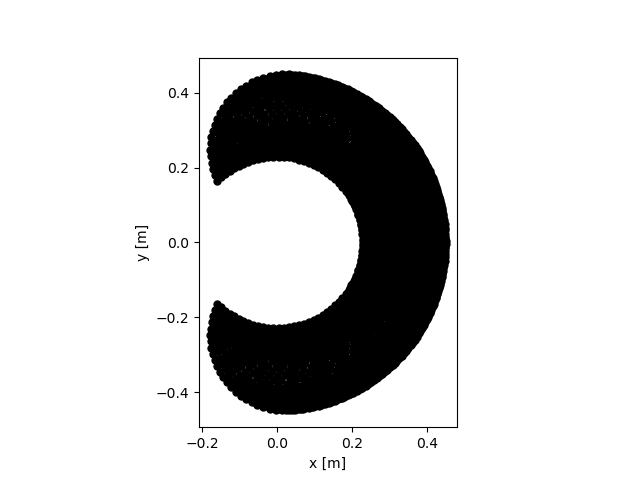
\includegraphics[width=0.6\linewidth]{pracovni_prostor.png}
    \caption{Dosažitelné polohy koncového bodu robota v rovině $xy$ základny (v rámci limitů
             kloubů $q_1$ a $q_2$).}
    \label{fig:prostor}
\end{figure}

% ---------------------------------------------------------------- 2 Přehled
\section{Přehled řešení}

Řešení má dvě fáze. Nejdřív robot z kamery zjistí, jak se deska s bludištěm otáčí, a předem
spočítá celý plán: pro každý krok čas příjezdu a konfiguraci, při které je střed obruče na
tyči. Potom plán projede, bez dalšího pozorování kamerou (obrázek~\ref{fig:prehled}).

\begin{figure}[ht]
\centering
\begin{tikzpicture}[
  box/.style={draw, rounded corners=3pt, minimum width=4.1cm, minimum height=1.25cm,
              align=center, font=\small},
  hl/.style={box, very thick, fill=blue!8},
  arr/.style={-{Stealth[length=2.2mm]}, thick}]
  \node[box] (snim) {\textbf{Snímání}\\ 22 snímků po 0{,}67\,s};
  \node[box, right=0.9cm of snim] (znac) {\textbf{Detekce značek}\\ ArUco 1 a 2, pixel $\to$ mm ($H$)};
  \node[box, right=0.9cm of znac] (otac) {\textbf{Odhad otáčení}\\ střed $C$, poloměr $r$, $\omega$, úhel $\alpha$};
  \node[box, below=1.6cm of snim] (draha) {\textbf{Dráha po tyči}\\ 77 bodů po 6{,}7\,mm};
  \node[hl,  below=1.6cm of znac] (plan) {\textbf{Plán}\\ IK, kolize, časy příjezdu ($3\times$)};
  \node[box, below=1.6cm of otac] (prov) {\textbf{Provedení}\\ pohyb odeslaný v čase $t - T$};
  \draw[arr] (snim) -- (znac);
  \draw[arr] (znac) -- (otac);
  \draw[arr] (otac.south) -- ++(0,-0.8) -| node[pos=0.25, above, font=\footnotesize] {poloha tyče v čase $t$} (plan.north);
  \draw[arr] (draha) -- (plan);
  \draw[arr] (plan) -- (prov);
\end{tikzpicture}
\caption{Průběh řešení: robot nejdřív spočítá celý plán, pak ho projede.}
\label{fig:prehled}
\end{figure}

Odhad otáčení dává plánu polohu každého bodu tyče v libovolném čase; plán k ní hledá
konfiguraci robota a čas příjezdu. Homografie $H$ pochází z kalibrace (kapitola~\ref{sec:kalibrace})
a doby pohybu z modelu změřeného předem (kapitola~\ref{sec:exp-model}).

% ---------------------------------------------------------------- 3 Kalibrace
\section{Kalibrace kamery a obruče}
\label{sec:kalibrace}

Kalibrace převádí pixely kamery na souřadnice $XY$ v základně robota [mm]. Využívá samotnou
obruč: robot ji postaví do 12 známých poloh, kamera najde její střed v obraze a ze dvojic
\uv{pixel $\leftrightarrow$ poloha z kinematiky} se spočítá homografie.

\subsection{Poloha obruče vůči koncovému bodu}

Knihovna robota vrací polohu koncového bodu (osy hřídele). Střed obruče je od ní posunutý
o vektor $D$ v souřadnicích koncového bodu:
\begin{equation}
  c = e + R(\varphi)\,D, \qquad D = 0{,}135\,\mathrm{m}\cdot(\cos 189^\circ,\ \sin 189^\circ),
\end{equation}
kde $e$ je poloha koncového bodu z přímé kinematiky a $\varphi = q_4$ je natočení koncového
bodu. U tohoto robota se $\varphi$ měří absolutně od osy $x$ základny, ne relativně k ramenům.
Délka 135\,mm je vzatá z dokumentace, úhel $189^\circ$ vyšel z fitu kalibračních dat
(kapitola~\ref{sec:exp-kalib}). Při plánování se používá opačný vztah $e = c - R(\varphi)D$:
pro zvolené natočení obruče se dopočítá, kde musí být koncový bod.

\subsection{Oprava nuly kloubu $q_2$}
\label{sec:q2}

Fit kalibračních dat ukázal, že úhel, který robot hlásí pro kloub $q_2$ (loket), se od
skutečného liší o stálou hodnotu:
\begin{equation}
  q_2^\mathrm{skut} = q_2^\mathrm{povel} + \Delta q_2, \qquad \Delta q_2 = 0{,}06\,\mathrm{rad} \approx 3{,}4^\circ .
\end{equation}
Bez opravy se střed obruče posune až o asi 1\,cm, a to různě podle natočení ramen. Inverzní
kinematika knihovny počítá se skutečným úhlem, takže robotu se posílá $q_2 - \Delta q_2$; při
kontrole kolize se naopak poloha ramene počítá ze skutečného úhlu $q_2 + \Delta q_2$
(konstanta \texttt{Q2\_OFF}).

\subsection{Snímání kalibračních poloh}

Skript \texttt{calibrate.py} projede 12 konfigurací (\texttt{CALIB\_Q}) ve výšce $q_3 = -0{,}23$.
V každé počká 0{,}5\,s na ustálení, uloží snímek a skutečné kloubové souřadnice. Polohy jsou
rozprostřené po celém záběru kamery a vybrané tak, aby rameno robota nezakrývalo obruč.

\subsection{Výpočet homografie}

Na každém snímku se střed obruče najde Houghovou transformací pro kružnice
(\texttt{cv2.HoughCircles} po mediánovém filtru). K němu se přiřadí poloha středu obruče
z přímé kinematiky:
\begin{align}
  x &= 250\cos q_1 + 200\cos(q_1+q_2) + 135\cos(q_4 + \delta),\\
  y &= 250\sin q_1 + 200\sin(q_1+q_2) + 135\sin(q_4 + \delta),
\end{align}
kde $\delta$ je úhel vektoru $D$. Z 12 dvojic se metodou nejmenších čtverců
(\texttt{cv2.findHomography}) spočítá homografie $H$, která mapuje pixel na $XY$ v mm.
Homografie platí pro rovinu, ve které byla obruč při kalibraci; ta je v rovině značek na desce.

\doplnit{finální program načítá \texttt{H\_angle\_candidate\_mm.npy}; uveďte, z jakých dat a
s jakým $\delta$ a $\Delta q_2$ vznikla. Pro konzistenci by měla být spočítaná se stejným modelem
obruče jako zbytek programu, např.\ \texttt{H\_fit\_mm.npy} z \texttt{fit\_calibration.py}.}

% ---------------------------------------------------------------- 4 Odhad otáčení
\section{Odhad otáčení stolku}
\label{sec:otaceni}

Z 22 snímků pořízených v rozestupu 0{,}67\,s (asi 14\,s) se určí střed otáčení, poloměr,
úhlová rychlost a natočení desky. Z nich lze pro libovolný čas $t$ spočítat, kde bude každý
bod tyče. Implementace je ve třídě \texttt{image\_proc} (\texttt{image\_processing.py}).

\subsection{Snímání a čas snímku}

Funkce \texttt{grab\_image()} při každém volání spustí snímání kamery, vezme první snímek,
přenese ho (asi 5\,Mpx) a snímání zastaví. Snímek tedy vzniká na začátku volání a zbytek je
přenos. Jako čas snímku se proto bere začátek volání $+$ \texttt{CAMERA\_DELAY} (0{,}03\,s),
ne střed volání.

\subsection{Detekce značek}

Na každém snímku se detektorem ArUco (\texttt{DICT\_4X4\_50}) najdou značky 1 a 2. Jejich rohy
se homografií převedou do roviny stolku a střed značky je průměr rohů. Snímky, na kterých
nejsou vidět obě značky (zakryje je rameno), se vynechají. Program pokračuje jen při
aspoň 8 platných snímcích. Jinak robot přejede do polohy pro focení a fotí znovu; pokud ani
pak nevidí obě značky na 8 snímcích, ukončí se s hlášením \uv{Aruco značky nejsou vidět}
ještě před zahájením jízdy.

\subsection{Střed otáčení, poloměr a natočení desky}

Střed desky $s$ je průměr středů obou značek. Ten při otáčení opisuje kružnici, která se
proloží algebraicky metodou nejmenších čtverců:
\begin{equation}
  x^2 + y^2 = 2ax + 2by + c \quad\Rightarrow\quad C = (a, b),\quad r = \sqrt{c + a^2 + b^2}.
\end{equation}
Značky jsou v protilehlých rozích čtverce, takže osa $x$ desky svírá s diagonálou (od značky 2
ke značce 1) úhel $45^\circ$. Úhel $\alpha$ mezi osou desky a spojnicí střed otáčení--střed
desky je pro tuhou desku stálý. Odhaduje se jako kruhový průměr přes všechny snímky.

\subsection{Úhlová rychlost a předpověď}
\label{sec:predpoved}

Úhel $\theta$ středu desky kolem středu otáčení se rozbalí (\texttt{np.unwrap}) a proloží
přímkou v čase. Směrnice je úhlová rychlost $\omega$ a absolutní člen je úhel v referenčním
čase $t_\mathrm{ref}$ (čas posledního platného snímku). Referenční úhel se bere z proložené
přímky přes všechny snímky, ne z jediného posledního snímku. Šum jednoho snímku by jinak
posunul celou předpověď.

Bod tyče $p_b$, zadaný v souřadnicích desky [mm], je v čase $t$ ve světě v bodě
\begin{equation}
  \theta(t) = \theta_\mathrm{ref} + \omega\,(t - t_\mathrm{ref}), \qquad
  p_w(t) = C + r\begin{pmatrix}\cos\theta(t)\\ \sin\theta(t)\end{pmatrix}
           + R\big(\theta(t) + \alpha\big)\,p_b .
\end{equation}
Výška bodu se nemění: $z = \texttt{Z\_PODLOZKA} + z_b$, kde $\texttt{Z\_PODLOZKA} = 0{,}27$\,m
je výška desky v souřadnicích robota.

\subsection{Geometrie tyče}
\label{sec:geometrie}

Tyč je zadaná lomenou čarou v souřadnicích desky [mm], od horního konce dolů a zpět nahoru:
\[
  (50, 50, 200) \to (50, 50, 150) \to (50, 0, 100) \to (0, 0, 50) \to (0, 0, 20)
  \to \text{zpět stejnou cestou}.
\]
Šikmé úseky leží ve dvou různých svislých rovinách, takže obruč se pohybuje ve všech třech
osách -- odtud varianta C.

% ---------------------------------------------------------------- 5 Plánování
\section{Plánování a provedení trajektorie}
\label{sec:plan}

Robot si nejdřív spočítá celý plán: pro každý krok čas příjezdu a kloubovou konfiguraci,
při které je střed obruče na tyči. Pak plán projede. Plán s předem spočítanými časy je
jednodušší než přepočítávání za jízdy a dobře se ladí.

\subsection{Rozdělení dráhy}

K lomené čáře tyče se na začátek přidá bod 30\,mm nad horním koncem (nájezd). Každý úsek se
rozdělí na kroky dlouhé nejvýš 6{,}7\,mm (\texttt{STEP\_MM}). Pro současnou tyč vznikne 77 bodů;
body 0--40 vedou dolů (bod 40 je nejnižší, 20\,mm nad podložkou), od bodu 41 se obruč vrací nahoru.

\subsection{Model doby pohybu}

Plán potřebuje vědět, jak dlouho bude robot do dalšího bodu jet. Doba pohybu se odhaduje
modelem změřeným skriptem \texttt{measure.py}: každý kloub se nezávisle posune o několik
různých vzdáleností a doba se proloží přímkou. Doba současného pohybu více kloubů je doba
nejpomalejšího z nich:
\begin{equation}
  T(\Delta q) = \max_j \left( a_j + \frac{|\Delta q_j|}{v_j} \right).
\end{equation}
Parametry pro relativní rychlost \texttt{SPEED} $= 0{,}5$ jsou v kapitole~\ref{sec:exp-model}.

\subsection{Inverzní kinematika a výběr řešení}

Obruč je osově souměrná, takže na jejím natočení nezáleží a pro jeden bod tyče existuje mnoho
konfigurací. Pro každé natočení $\varphi$ z mřížky po $5^\circ$ se spočítá poloha koncového
bodu $e = c - R(\varphi)D$ a zavolá se inverzní kinematika knihovny (\texttt{robot.ik}). Ta
vrátí až dvě polohy lokte a více variant $q_4$ ($\varphi + 2k\pi$ v rozsahu kloubu). Každé
řešení se opraví o $\Delta q_2$ (kapitola~\ref{sec:q2}) a vyřadí se řešení mimo limity kloubů
a řešení, která kolidují s tyčí (kapitola~\ref{sec:kolize}).

Ze zbylých se vybere to nejbližší předchozímu kroku (nejmenší $\|q - q_\mathrm{prev}\|$).
Po dráze platí dvě omezení:
\begin{itemize}
  \item \textbf{$q_4$ se za krok otočí nejvýš o $30^\circ$} (\texttt{MAX\_DPHI}). Jinak by výběr
        mohl zvolit stejnou polohu s $q_4$ o $360^\circ$ jinak a robot by se otočil dokola;
  \item \textbf{loket nesmí přeskočit na druhou stranu}. Přeskok by znamenal velký pohyb
        celého ramene nad bludištěm.
\end{itemize}
Pro první bod (nájezd nad tyč) se vybere natočení, při kterém je kolidující díl co nejdál
od tyče.

\subsection{Časování plánu}

Kam má robot jet, závisí na čase příjezdu, a čas příjezdu závisí na tom, jak daleko robot
jede. Plán se proto počítá třikrát:
\begin{enumerate}
  \item odhadnou se časy příjezdu $t_i$ do všech bodů;
  \item pro každý bod se spočítá poloha tyče v čase $t_i + \texttt{LEAD\_T}$ a vybere konfigurace;
  \item z modelu doby pohybu se určí rozestupy kroků $1{,}1\,T + 0{,}05$\,s a nové časy.
        Začátek se posune tak, aby robot stihl výpočet a příjezd na první bod.
\end{enumerate}
\texttt{LEAD\_T} vyrovnává stálé zpoždění mezi skutečnou polohou desky a předpovědí
(zpoždění kamery, reakce robota). Kladná hodnota míří tam, kde tyč bude později, záporná
dříve. Ve finální verzi se nastavuje podle směru otáčení a polohy stolku
(tabulka~\ref{tab:lead}); hodnoty byly nalezeny experimentálně (kapitola~\ref{sec:exp-lead}).

\begin{table}[ht]
\centering
\begin{tabular}{@{}l r r@{}}
\toprule
 & střed otáčení $y \le 0$ & střed otáčení $y > 0$ \\
\midrule
$\omega < 0$ & $+0{,}05$\,s & $\phantom{+}0{,}00$\,s \\
$\omega \ge 0$ & $-0{,}03$\,s & $-0{,}08$\,s \\
\bottomrule
\end{tabular}
\caption{Hodnota \texttt{LEAD\_T} podle směru otáčení stolku a strany, na které stolek leží.}
\label{tab:lead}
\end{table}

\subsection{Nedosažitelná poloha}

Pokud pro některý bod dráhy neexistuje konfigurace v limitech kloubů bez kolize, výpočet plánu
skončí výpisem \uv{Plán selhal: bod $i$ nemá řešení IK \ldots}. Protože některá selhání závisí
na natočení stolku v okamžiku příjezdu (kolize dílu u hřídele s tyčí), program pak desku znovu
nafotí a plán spočítá ještě jednou. Pokud selže i druhý plán, vypíše \uv{Bludiště je v této
poloze nedosažitelné, nepohybuji se.} a robot se k bludišti vůbec nerozjede. Nedosažitelnost
je tak nahlášena ještě před zahájením pohybu, jak požaduje zadání.

\subsection{Provedení plánu}

Každý pohyb se odešle v čase $t_i - T_i$ (\texttt{move\_to\_q}), aby robot dojel přesně
v plánovaný čas, a pak se počká na zastavení (\texttt{wait\_for\_motion\_stop}). Na konci se
vypíše, o kolik se robot od plánu zpozdil.

Nejnižší bod dráhy je 20\,mm nad podložkou, tedy pod hranicí 4\,cm z kritéria úspěchu. Dráha
pak pokračuje po tyči zpět nahoru, takže robot na konci bezpečně vyjede svisle nahoru
a vrátí se domů, aniž by obruč táhl přes tyč.

Celý pokus trvá zhruba \doplnit{změřit; odhad: 15\,s focení $+$ asi 1\,s plán $+$ asi
40\,s jízda}, tedy pod limitem 2 minut.

% ---------------------------------------------------------------- 6 Kolize
\section{Kolize robota s bludištěm}
\label{sec:kolize}

Obruč sama do tyče nenarazí, pokud je její střed na tyči. Do tyče ale narážel malý svislý
váleček na příchytce vedle hřídele. Plán proto vyřazuje konfigurace, ve kterých by se tento
díl dostal k tyči.

\subsection{Model kolidujícího dílu}

Ramena a loket jsou podle výkresu robota výš než vršek tyče, takže do ní narazit nemohou.
Kolidující díl je přichycený k hřídeli a jezdí nahoru a dolů spolu s obručí. V půdorysu ho
modelujeme jako svislý válec (tabulka~\ref{tab:dil}).

\begin{table}[ht]
\centering
\begin{tabularx}{\linewidth}{@{}l r X@{}}
\toprule
parametr & hodnota & význam \\
\midrule
\texttt{HOUSING\_OFFSET} & 85\,mm & vzdálenost středu dílu od osy hřídele \\
\texttt{HOUSING\_ANGLE} & $157^\circ$ & směr od osy hřídele, měřený od směru ramene 2 (loket $\to$ hřídel);
  díl je mezi loktem a hřídelí, $23^\circ$ vlevo \\
\texttt{HOUSING\_R} & 35\,mm & poloměr dílu $+$ poloměr tyče $+$ rezerva \\
\texttt{HOUSING\_DZ} & 30\,mm & o kolik je spodek dílu výš než rovina obruče \\
\bottomrule
\end{tabularx}
\caption{Model kolidujícího dílu.}
\label{tab:dil}
\end{table}

Díl je pevně na rameni 2, takže se neotáčí s $q_4$. Jeho střed je v bodě
$e + \texttt{HOUSING\_OFFSET}\cdot(\cos\beta, \sin\beta)$, kde
$\beta = q_1 + q_2^\mathrm{skut} + \texttt{HOUSING\_ANGLE}$.

\subsection{Kontrola kolize}

Tyč se navzorkuje body po 5\,mm, včetně svislého kusu od spodního bodu dráhy až na desku, kde
je tyč uchycená. Pro kandidátní konfiguraci a čas příjezdu se tyč posune do světa
(kapitola~\ref{sec:predpoved}). Kontrolují se jen body tyče, které jsou výš než spodek dílu.
Konfigurace koliduje, pokud je některý z nich vodorovně blíž než \texttt{HOUSING\_R} od
středu dílu.

Kolize se kontrolují jen na cestě dolů (body 0--40). Cestou nahoru robot jede po stejné tyči
a kontrola tam zbytečně vyřazovala řešení a vedla k nuceným otočkám $q_4$. Omezení
z kapitoly~\ref{sec:plan} (nejvýš $30^\circ$ za krok, bez přeskoku lokte) platí i cestou nahoru.

\subsection{Závislost na směru otáčení}
\label{sec:smer}

Výběr nejbližší konfigurace má nepříjemnou vlastnost: když se kolizní oblast kvůli otáčení
desky posouvá k aktuálnímu natočení, robot se odtočí jen o tolik, aby z ní vyklouzl, a jede
po hraně kolize. Záleží na směru otáčení stolku, proto robot během vývoje při jednom směru
narážel a při druhém ne. To je podstatné pro bonus za oba směry otáčení. Zmírnili jsme to
dostatečnou rezervou v \texttt{HOUSING\_R} (35\,mm) a laděním \texttt{LEAD\_T} zvlášť pro
každý směr (tabulka~\ref{tab:lead}).

% ---------------------------------------------------------------- 7 Experimenty
\section{Experimenty}

Experimenty sloužily k určení parametrů (model doby pohybu, kalibrace, časový předstih)
a k ověření, kde řešení funguje. Některé varianty plánovače jsme nejdřív zkoušeli v simulaci:
robot nahrazený objektem s kinematikou z knihovny (\texttt{RobotBosch(tty\_dev=None)}) a dobou
pohybu podle modelu, stolek s náhodnou polohou, poloměrem a rychlostí otáčení.

\subsection{Model doby pohybu}
\label{sec:exp-model}

Skript \texttt{measure.py} pohnul každým kloubem třikrát o tři různé vzdálenosti ($q_1$, $q_2$:
0{,}1 / 0{,}2 / 0{,}4\,rad; $q_3$: 2 / 5 / 10\,cm; $q_4$: 0{,}2 / 0{,}5 / 1\,rad) a měřil dobu
od \texttt{move\_to\_q} do konce \texttt{wait\_for\_motion\_stop}. Proložení přímkou dalo pro
\texttt{SPEED} $= 0{,}5$ hodnoty v tabulce~\ref{tab:model}.

\begin{table}[ht]
\centering
\begin{tabular}{@{}l r r@{}}
\toprule
kloub & $a_j$ [s] & $v_j$ \\
\midrule
$q_1$ & 0{,}214 & 0{,}396\,rad/s \\
$q_2$ & 0{,}216 & 0{,}620\,rad/s \\
$q_3$ & 0{,}175 & 0{,}0263\,m/s \\
$q_4$ & 0{,}135 & 0{,}518\,rad/s \\
\bottomrule
\end{tabular}
\caption{Parametry modelu doby pohybu.}
\label{tab:model}
\end{table}

Na šesti náhodných pohybech více kloubů najednou se model od měření lišil nejvýš o 6{,}1\,\%.
Nejpomalejší je svislý posuv $q_3$: krok 6{,}7\,mm svisle trvá asi 0{,}43\,s, vodorovný krok
stejné délky méně.

\subsection{Přesnost kalibrace}
\label{sec:exp-kalib}

Na 12 kalibračních snímcích jsme porovnali polohu obruče nalezenou v obraze s polohou
z kinematiky a nechali dofitovat model obruče. Chyba na snímku vynechaném z fitu
(leave-one-out) je v tabulce~\ref{tab:kalib}.

\begin{table}[ht]
\centering
\begin{tabular}{@{}l r r@{}}
\toprule
model obruče & střední chyba & max.\ chyba \\
\midrule
$D = 135$\,mm pod $185^\circ$, bez dalších oprav & 5{,}4\,mm & 10{,}1\,mm \\
dofitované $D$ & 2{,}7\,mm & 6{,}1\,mm \\
dofitované $D$ $+$ posun nuly kloubu $q_2$ & 0{,}75\,mm & 1{,}7\,mm \\
\bottomrule
\end{tabular}
\caption{Chyba modelu obruče na kalibračních snímcích.}
\label{tab:kalib}
\end{table}

Nejlepší model vyšel $D = 134{,}3$\,mm pod $\approx 189^\circ$ a posun $q_2$ o $+3{,}4^\circ$.
Chyba asi 1\,cm v původním modelu stačí na to, aby obruč minula střed tyče. Finální program
proto používá $D$ pod $189^\circ$ a opravu $\Delta q_2 = 0{,}06$\,rad (kapitola~\ref{sec:q2}).
\doplnit{jak se oprava projevila na robotu}

\subsection{Časový předstih \texttt{LEAD\_T}}
\label{sec:exp-lead}

\texttt{LEAD\_T} se ladil na robotu: když tyč tlačila na přední stranu obruče ve směru otáčení,
předstih se zvýšil, a naopak. Chyba časování je nejvíc vidět na částech tyče daleko od osy
stolku. Ukázalo se, že nejlepší hodnota závisí na směru otáčení a na tom, na které straně
pracovního prostoru stolek leží; výsledné hodnoty jsou v tabulce~\ref{tab:lead}. Závislost na
straně je pravděpodobně zbytková chyba geometrie (kalibrace), kterou časový posun částečně
vyrovná.

Během ladění jsme pozorovali, že pro stejnou polohu stolku občas fungovalo $+0{,}2$\,s
i $-0{,}2$\,s, ale ne 0. Čistá chyba časování by se takhle chovat nemohla, protože oba posuny
posouvají obruč na opačné strany tyče. Příčinou byl rozptyl mezi jednotlivými spuštěními:
referenční úhel desky se bral z jediného snímku. Po přechodu na úhel z proložené přímky
(kapitola~\ref{sec:predpoved}) a prodloužení focení na 22 snímků byly výsledky stabilnější.
\doplnit{případně tabulka zkoušených hodnot \texttt{LEAD\_T}}

\subsection{Kolize s bludištěm}

Na robotu se ukázalo, že do tyče nenarážejí ramena, ale díl u hřídele (kapitola~\ref{sec:kolize}).
Další zjištění:
\begin{itemize}
  \item \textbf{Otočky o $360^\circ$:} bez limitu pootočení $q_4$ si plán občas vybral stejnou
        polohu s $q_4$ o otočku jinak a robot držákem smetl tyč. Limit $30^\circ$ na krok to
        odstranil.
  \item \textbf{Závislost na směru otáčení:} při jednom směru otáčení stolku robot narážel, při
        druhém ne (vysvětlení v kapitole~\ref{sec:smer}).
  \item \textbf{Selhání plánu:} výběr krok po kroku vidí jen jeden krok dopředu. V simulaci na
        40 náhodných scénářích plán selhal v 5 případech, přestože bezkolizní řešení
        existovalo. Proto program při selhání plán jednou zopakuje s novými snímky.
\end{itemize}

\subsection{Kde řešení funguje}

Zadání doporučuje zobrazit, ve kterých částech pracovního prostoru řešení funguje. Stolek jsme
postupně umístili do šesti poloh pro každý směr otáčení a v každé provedli dva pokusy
(tabulka~\ref{tab:mapa}, obrázek~\ref{fig:mapa}). Poloha stolku je střed otáčení vypsaný
programem.

\begin{table}[ht]
\centering
\begin{tabular}{@{}l r c c@{}}
\toprule
poloha $(x, y)$ [mm] & $\omega$ [$^\circ$/s] & pokusů & úspěšných \\
\midrule
\multicolumn{4}{@{}l}{\textit{otáčení $\omega < 0$}} \\
(365, 86) & $-12{,}8$ & 2 & 2 \\
(265, 110) & $-12{,}7$ & 2 & 2 \\
(390, $-$21) & $-12{,}9$ & 2 & 2 \\
(233, 18) & $-12{,}9$ & 2 & 2 \\
(245, $-$146) & $-12{,}8$ & 2 & 2 \\
(388, $-$162) & $-12{,}7$ & 2 & 2 \\
\midrule
\multicolumn{4}{@{}l}{\textit{otáčení $\omega > 0$}} \\
(365, 84) & $+13{,}0$ & 2 & 2 \\
(267, 115) & $+13{,}0$ & 2 & 2 \\
(411, $-$18) & $+12{,}6$ & 2 & 2 \\
(397, $-$122) & $+12{,}7$ & 2 & 2 \\
(255, $-$173) & $+12{,}6$ & 2 & 2 \\
(232, 17) & $+12{,}6$ & 2 & 2 \\
\bottomrule
\end{tabular}
\caption{Úspěšnost řešení v pracovní ploše pro oba směry otáčení.}
\label{tab:mapa}
\end{table}

\begin{figure}[ht]
    \centering
    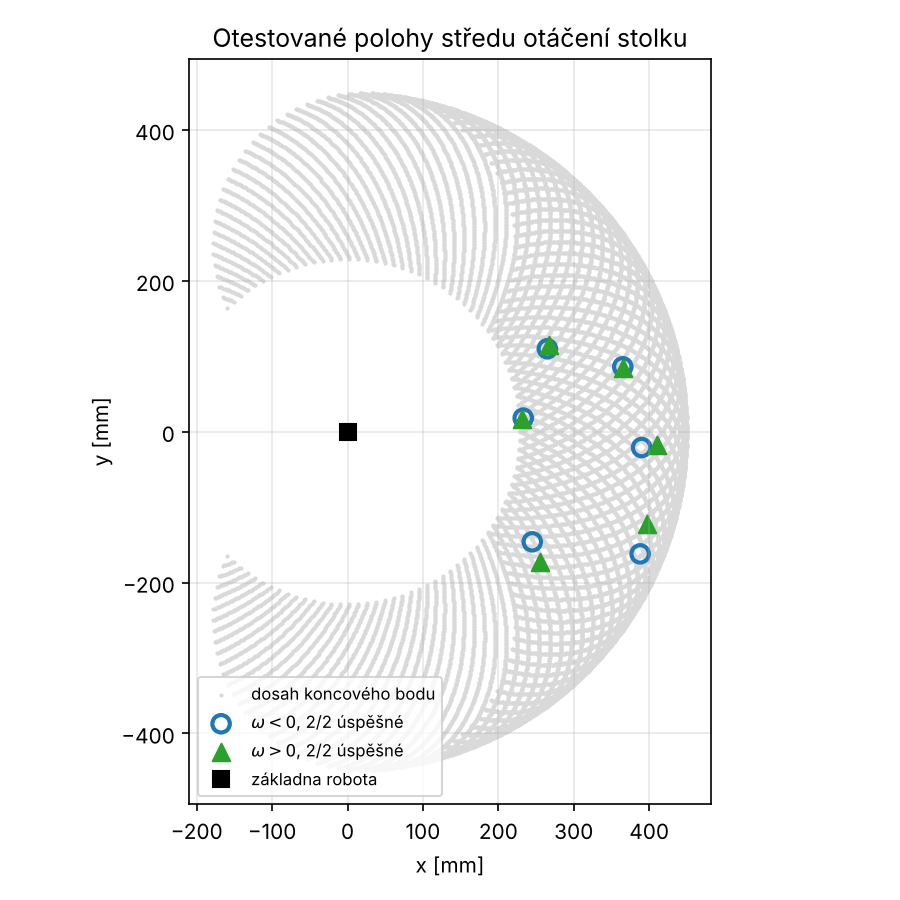
\includegraphics[width=0.62\linewidth]{mapa.png}
    \caption{Otestované polohy středu otáčení stolku na pozadí dosahu koncového bodu robota.
             Kroužky: $\omega < 0$, trojúhelníky: $\omega > 0$.}
    \label{fig:mapa}
\end{figure}

Řešení uspělo ve všech 24 pokusech, tedy ve všech testovaných polohách v obou směrech otáčení.
V poloze nejdál od základny, $(411, -18)$\,mm, robot při jednom pokusu zavadil o ochranné sklo
pracoviště. Pokus přesto skončil úspěšně, ukazuje to ale, že tato poloha je na hraně bezpečně
použitelného prostoru.

% ---------------------------------------------------------------- 8 Implementace
\section{Implementace a spuštění}

Řešení je napsané v Pythonu nad knihovnami \texttt{ctu\_bosch\_sr450}, OpenCV a NumPy. Hlavní
program se spouští příkazem \texttt{python main\_finalized.py} z adresáře projektu, kde musí
být \texttt{duration\_model.json} a soubor s homografií.

\begin{table}[ht]
\centering
\begin{tabularx}{\linewidth}{@{}l X@{}}
\toprule
soubor & obsah \\
\midrule
\texttt{main\_finalized.py} & hlavní program: snímání, plán, kolize, provedení \\
\texttt{image\_processing.py} & detekce značek, odhad otáčení, předpověď polohy tyče, body tyče \\
\texttt{calibrate.py} & kalibrační polohy, výpočet homografie, natočení $q_4$ do středu rozsahu \\
\texttt{fit\_calibration.py} & fit modelu obruče a posunu $q_2$ z kalibračních snímků \\
\texttt{measure.py} & měření modelu doby pohybu \\
\texttt{duration\_model.json} & změřené parametry $a_j$, $v_j$ \\
\bottomrule
\end{tabularx}
\caption{Struktura kódu.}
\end{table}

Po inicializaci robot natočí $q_4$ na $360^\circ$ (\texttt{fix\_negative\_uhel}), aby měl na obě
strany rezervu na otáčení obruče. Celá jízda je v bloku \texttt{try/finally}, takže se robot
i při chybě vrátí domů a spojení se uzavře. Když plán nenajde řešení ani na druhý pokus,
robot se k bludišti nerozjede.

% ---------------------------------------------------------------- 9 Diskuze
\section{Diskuze}

Řešení stojí na jednoduchém principu: předpovědět, kde bude tyč, a dojet tam ve správný čas.
Přesnost je dána hlavně třemi zdroji chyb:
\begin{itemize}
  \item \textbf{Kalibrace:} model obruče a homografie. Oprava kloubu $q_2$ zmenšila chybu modelu
        obruče z jednotek milimetrů pod 2\,mm (tabulka~\ref{tab:kalib}).
  \item \textbf{Odhad otáčení:} chyba úhlové rychlosti roste lineárně s délkou jízdy, chyba fáze
        se projeví nejvíc daleko od osy stolku.
  \item \textbf{Časování:} stálé zpoždění kamery a robota je vyrovnané ručně laděným
        \texttt{LEAD\_T}. Hodnota se nedala odvodit z měření kamerou, protože ta má stejné zpoždění.
\end{itemize}

Další omezení:
\begin{itemize}
  \item \textbf{Plán bez výhledu dopředu:} výběr konfigurace krok po kroku může skončit v bodě,
        odkud nevede bezkolizní pokračování do $30^\circ$. Dynamické programování přes celou
        dráhu by to odstranilo (v simulaci 0 selhání ze 40), ale výpočet plánu by trval asi 4\,s
        místo 0{,}6\,s.
  \item \textbf{Zjednodušený model kolize:} hlídá se jen jeden díl u hřídele a jen v cílové
        poloze kroku, ne během přejezdu mezi kroky. Ochranné sklo pracoviště se nehlídá vůbec.
  \item \textbf{Pohyb se zastavováním:} robot se po každém kroku zastaví. Deska se mezitím otáčí
        dál, takže mezi kroky obruč nepřesně sleduje tyč.
  \item \textbf{Ruční \texttt{LEAD\_T} podle strany a směru:} funguje v otestovaných polohách,
        ale jde o empirickou korekci, ne o odstranění příčiny.
\end{itemize}

Možná vylepšení: homografie spočítaná se stejným modelem obruče jako plánování, plánování
dynamickým programováním, hlídání vzdálenosti od skla, pohyby ve frontě řízení bez
zastavování a průběžná oprava fáze stolku z dalších snímků během jízdy.

% ---------------------------------------------------------------- Závěr
\section{Závěr}

Robot Bosch SR450 provléká obruč po tyči bludiště na otáčejícím se stolku tak, že z kamery
odhadne otáčení desky, předem spočítá časovaný plán konfigurací a ten projede. Plán hlídá
limity kloubů, plynulost natočení obruče a kolizi dílu u hřídele s tyčí. Experimenty určily
model doby pohybu, opravu kloubu $q_2$ a časový předstih pro oba směry otáčení. Řešení
uspělo ve všech 24 pokusech ve 12 polohách stolku v obou směrech otáčení; v poloze nejdál
od základny se robot jednou dotkl ochranného skla. Nedosažitelnou polohu bludiště i chybějící
značky program nahlásí před zahájením pohybu.

% ---------------------------------------------------------------- Podíl členů
\section{Podíl členů týmu na technickém řešení}

\doplnit{celá kapitola}. Tým má tři členy. Zadání vyžaduje, aby každý člen měl technický přínos a uměl ho při
předvádění vysvětlit; rozdělení \uv{implementace vs.\ psaní zprávy} nestačí. Návrh rozdělení
podle částí řešení je v tabulce~\ref{tab:podil}.

\begin{table}[ht]
\centering
\begin{tabularx}{\linewidth}{@{}l l X@{}}
\toprule
člen týmu & technická část & konkrétně \\
\midrule
\doplnit{} & kalibrace kamery a obruče & \doplnit{např.\ \texttt{calibrate.py}, výběr kalibračních poloh, homografie, oprava $q_2$} \\
\doplnit{} & zpracování obrazu a odhad otáčení & \doplnit{např.\ \texttt{image\_processing.py}, ArUco, fit kružnice a $\omega$} \\
\doplnit{} & plánování, IK a kolize & \doplnit{např.\ \texttt{main\_finalized.py}, model doby pohybu, kontrola kolize} \\
\doplnit{} & experimenty a ladění & \doplnit{např.\ \texttt{measure.py}, ladění \texttt{LEAD\_T}, mapa pracovní plochy} \\
\bottomrule
\end{tabularx}
\caption{Podíl členů týmu.}
\label{tab:podil}
\end{table}

% ---------------------------------------------------------------- AI
\section{Využití AI při implementaci a psaní zprávy}

\doplnit{ověřit a upravit podle skutečnosti; případně doplnit další nástroje, které tým používal}

\begin{itemize}
  \item \textbf{Analýza kódu a hledání chyb (Claude):} AI procházela naše skripty a upozorňovala
        na slabá místa, např.\ nekonzistentní časování mezi plánem a provedením, chybný směr
        držáku obruče v kontrole kolize nebo otočky $q_4$ o $360^\circ$. To bylo nejpřínosnější
        použití.
  \item \textbf{Diagnostika z dat:} AI z kalibračních snímků spočítala chybu modelu obruče
        a navrhla opravu kloubu $q_2$ (tabulka~\ref{tab:kalib}). V simulaci ověřovala, kdy plán
        selže a proč.
  \item \textbf{Návrh kódu:} zjednodušení hlavního programu, kontrola kolize kolidujícího dílu
        a výběr kalibračních poloh. Geometrické rozměry (poloha dílu, $D$, \texttt{Z\_PODLOZKA})
        a finální hodnoty parametrů jsme měřili a ladili na robotu sami.
  \item \textbf{Psaní zprávy:} první verzi textu napsala AI podle kódu a průběhu vývoje; tým ji
        zkontroloval a doplnil měření a podíl členů.
  \item \textbf{Zkušenost:} AI byla silná v rychlé analýze a simulaci, ale bez znalosti
        skutečného robota někdy předpokládala špatnou geometrii (např.\ že do tyče naráží osa
        hřídele, ne díl vedle ní). Návrhy proto bylo nutné ověřovat na robotu.
\end{itemize}

\end{document}
